\documentclass[conference,a4paper]{IEEEtran}

% ── Packages ──────────────────────────────────────────────────────────────────
\usepackage[T1]{fontenc}
\usepackage[utf8]{inputenc}
\usepackage{graphicx}
\usepackage{booktabs}
\usepackage{amsmath}
\usepackage{amssymb}
\usepackage[hidelinks]{hyperref}
\usepackage{cite}
\usepackage{microtype}
\usepackage{xcolor}
\usepackage{caption}
\usepackage{subcaption}
\usepackage{float}
\usepackage{enumitem}
\usepackage{multirow}
\usepackage{url}
\usepackage{balance}

\graphicspath{{./}}

\title{ExplainRAG: Confidence-Calibrated Hybrid RAG\\
for Healthcare Question Answering}

\author{
  \IEEEauthorblockN{Kalaivani K}
  \IEEEauthorblockA{
    \textit{Assistant Professor Sr. Grade 2}\\
    \textit{Department of Database Systems, SCOPE}\\
    \textit{VIT University}\\
    Vellore, India\\
    kalaivani.k@vit.ac.in
  }
  \and
  \IEEEauthorblockN{Kasilanka Bhoopesh Siva Srikar}
  \IEEEauthorblockA{
    \textit{School of Computer Science and Engineering (SCOPE)}\\
    \textit{VIT University}\\
    Vellore, India\\
    22BCE0580\\
    kasilanka.bhoopesh2022@vitstudent.ac.in
  }
}

\begin{document}

\maketitle

% ── Abstract ──────────────────────────────────────────────────────────────────
\begin{abstract}
Large language models deployed for healthcare question answering face
two persistent failure modes: hallucination of plausible but incorrect
medical claims, and opacity---the system gives no evidence trail,
so the user cannot assess reliability.
This paper describes a locally deployable healthcare QA system that
addresses both by combining hybrid retrieval-augmented generation (RAG)
with a five-signal explainable AI (XAI) confidence layer.

The knowledge base contains 505,584 sentence-boundary-aware chunks drawn
from PubMedQA, MedMCQA, and the ChatDoctor-HealthCareMagic patient-doctor
dialogue corpus.
Queries are answered by fusing BM25 sparse retrieval with dense vector
search (all-MiniLM-L6-v2, ChromaDB) using Reciprocal Rank Fusion (RRF),
then generating a response with TinyLlama-1.1B or BioMistral-7B.
Every response carries source attributions, a Platt-calibrated confidence
score, and a DeBERTa-v3 hallucination flag.

On 97 held-out medical questions (bootstrap 95\% CIs), the full system
achieves keyword coverage 0.385 [0.32--0.46] and ROUGE-L 0.208
[0.17--0.25], a 63\% gain over the no-RAG baseline (keyword coverage
0.236).
A QLoRA-adapted TinyLlama reaches keyword coverage 0.463, a 20\% relative
improvement.
Ablation shows that the source-agreement signal intentionally reduces raw
keyword coverage by 6.1 points when retrieved sources conflict rather than
asserting a single answer---a safety-oriented tradeoff that standard QA
benchmarks do not capture.
Calibration ECE is 0.14 on the same 97-question set.
All code, evaluation scripts, and the knowledge base build pipeline are
openly available.
\end{abstract}

\begin{IEEEkeywords}
healthcare question answering, retrieval-augmented generation,
hybrid retrieval, explainable AI, confidence calibration,
small language models, biomedical NLP, QLoRA
\end{IEEEkeywords}

% ── 1. Introduction ───────────────────────────────────────────────────────────
\section{Introduction}
\label{sec:intro}

Large language models (LLMs) are increasingly used as consumer-facing
health information tools, yet two failure modes remain unsolved at scale.
The first is hallucination: the model generates plausible but factually
incorrect medical claims without any mechanism that would alert the user.
The second is opacity: the response provides no evidence trail, so a
patient cannot verify what the system is saying or decide how much weight
to give it \cite{singhal2023large,thirunavukarasu2023}.

Retrieval-augmented generation (RAG) \cite{lewis2020rag} directly
addresses hallucination by grounding generation in documents retrieved
at query time.
Explainable AI (XAI) addresses opacity by surfacing the evidence and
quantifying how confident the system is \cite{amann2020xai}.
Published work has explored each approach in medical NLP independently,
but combining both in a single system---with real calibration experiments
on held-out data---is uncommon in the open-source RAG literature.

A practical constraint motivates the choice of TinyLlama-1.1B
\cite{zhang2024tinyllama}: most published systems assume GPU
availability for both retrieval and generation, but TinyLlama runs at
acceptable speed on CPU hardware that most students and small clinics
already own.
This makes it a feasible but slow default for a privacy-preserving local
deployment where queries never leave the user's machine.

The primary scientific contribution of this work is the integration of
hybrid RAG with a calibrated, multi-signal XAI layer that quantifies
trust in real time. We make the following specific contributions:

\begin{enumerate}[noitemsep,topsep=2pt]
  \item \textbf{Scientific Contributions:} We demonstrate a hybrid retrieval
        pipeline fused via query-type-adaptive RRF. We introduce a five-signal
        XAI confidence layer with Platt-scaled calibration and a DeBERTa-v3
        NLI hallucination gate. Our ablation study hypothesises that
        source-agreement constraints intentionally reduce raw extraction
        metrics in favor of safer abstention.
  \item \textbf{Engineering Artifacts:} We provide a QLoRA adapter
        fine-tuned on medical Q\&A that improves keyword coverage by 20\%,
        and package the local-first FastAPI/React system into a reproducible
        Docker Compose setup.
\end{enumerate}

The rest of the paper is organised as follows.
Section~\ref{sec:related} reviews prior work.
Section~\ref{sec:arch} describes the system architecture and pipeline.
Section~\ref{sec:xai} covers the XAI methodology.
Section~\ref{sec:eval} presents evaluation results.
Section~\ref{sec:discussion} discusses the findings.
Section~\ref{sec:limitations} acknowledges limitations.
Section~\ref{sec:conclusion} concludes with future directions.

% ── 2. Related Work ───────────────────────────────────────────────────────────
\section{Related Work}
\label{sec:related}

\subsection{RAG for medical QA}

Lewis et al.\ \cite{lewis2020rag} introduced RAG as a general
framework; subsequent work adapted it for biomedical QA using
domain-specific retrievers including BM25 \cite{robertson2009bm25}
and dense passage retrieval \cite{karpukhin2020dpr}.
Jin et al.\ \cite{jin2023medcpt} proposed MedCPT, a contrastive
retriever pre-trained on PubMed search logs.
Our system uses all-MiniLM-L6-v2 for dense retrieval rather than
a domain-specific encoder, which allows us to avoid dependency on
a proprietary embedding model while still achieving competitive
retrieval quality.

\subsection{Medical language models}

Singhal et al.\ \cite{singhal2023large} showed that large LLMs can pass
USMLE-style exams but noted persistent calibration problems.
BioMistral \cite{labrak2024biomistral} continues pre-training Mistral-7B
on PubMed Central Open Access articles and reaches 59.1\% on MedMCQA.
ChatDoctor \cite{li2023chatdoctor} is a LLaMA-based model fine-tuned on
patient-doctor dialogues; we use its training corpus as one of three knowledge
base sources.
TinyLlama \cite{zhang2024tinyllama} is not a medical model, but at 1.1B
parameters in bfloat16 it is the only candidate that runs at tolerable
speed on CPU without quantisation.

\subsection{Hybrid retrieval}

Combining sparse (BM25) and dense retrieval consistently outperforms
either method alone on open-domain QA benchmarks \cite{ma2022hybrid}.
Cormack et al.\ \cite{cormack2009rrf} proposed Reciprocal Rank Fusion
as a score-normalisation-free way to merge ranked lists.
Our system extends standard RRF with query-type detection that adjusts
the dense-to-sparse weight ratio depending on whether the query asks about
a drug, a definition, a symptom, or a comparison.

\subsection{Confidence calibration and XAI}

Guo et al.\ \cite{guo2017calibration} showed that modern neural networks
are poorly calibrated and proposed temperature scaling as a post-hoc fix.
Platt scaling \cite{platt1999probabilistic} is a logistic-regression
variant that works well on small calibration sets.
Tjoa and Guan \cite{tjoa2020survey} survey post-hoc versus intrinsic
explainability methods for clinical AI; Amann et al.\ \cite{amann2020xai}
find that citation-based explanations are most valued by clinicians.
Our system provides both: per-source span attribution and a numeric
multi-signal confidence score.

\subsection{Positioning}

Recent RAG systems for medical QA include MedRAG \cite{xiong2024medrag},
which benchmarks retrieval corpora on four medical QA datasets, and
domain-specific retrievers such as MedCPT \cite{jin2023medcpt}.
These systems focus on retrieval and generation quality but do not
provide calibrated confidence scores or hallucination flags alongside
each response.
On the XAI side, published clinical explainability work addresses
feature attribution for diagnostic models \cite{tjoa2020survey} rather
than grounding trust signals in a live retrieval pipeline.
To our knowledge, no prior open-source system integrates hybrid RAG
with a calibrated multi-signal XAI layer for medical question answering;
this combination is the central contribution of the present work.

% ── 3. System Architecture ────────────────────────────────────────────────────
\section{System Architecture}
\label{sec:arch}

\begin{figure}[t]
  \centering
  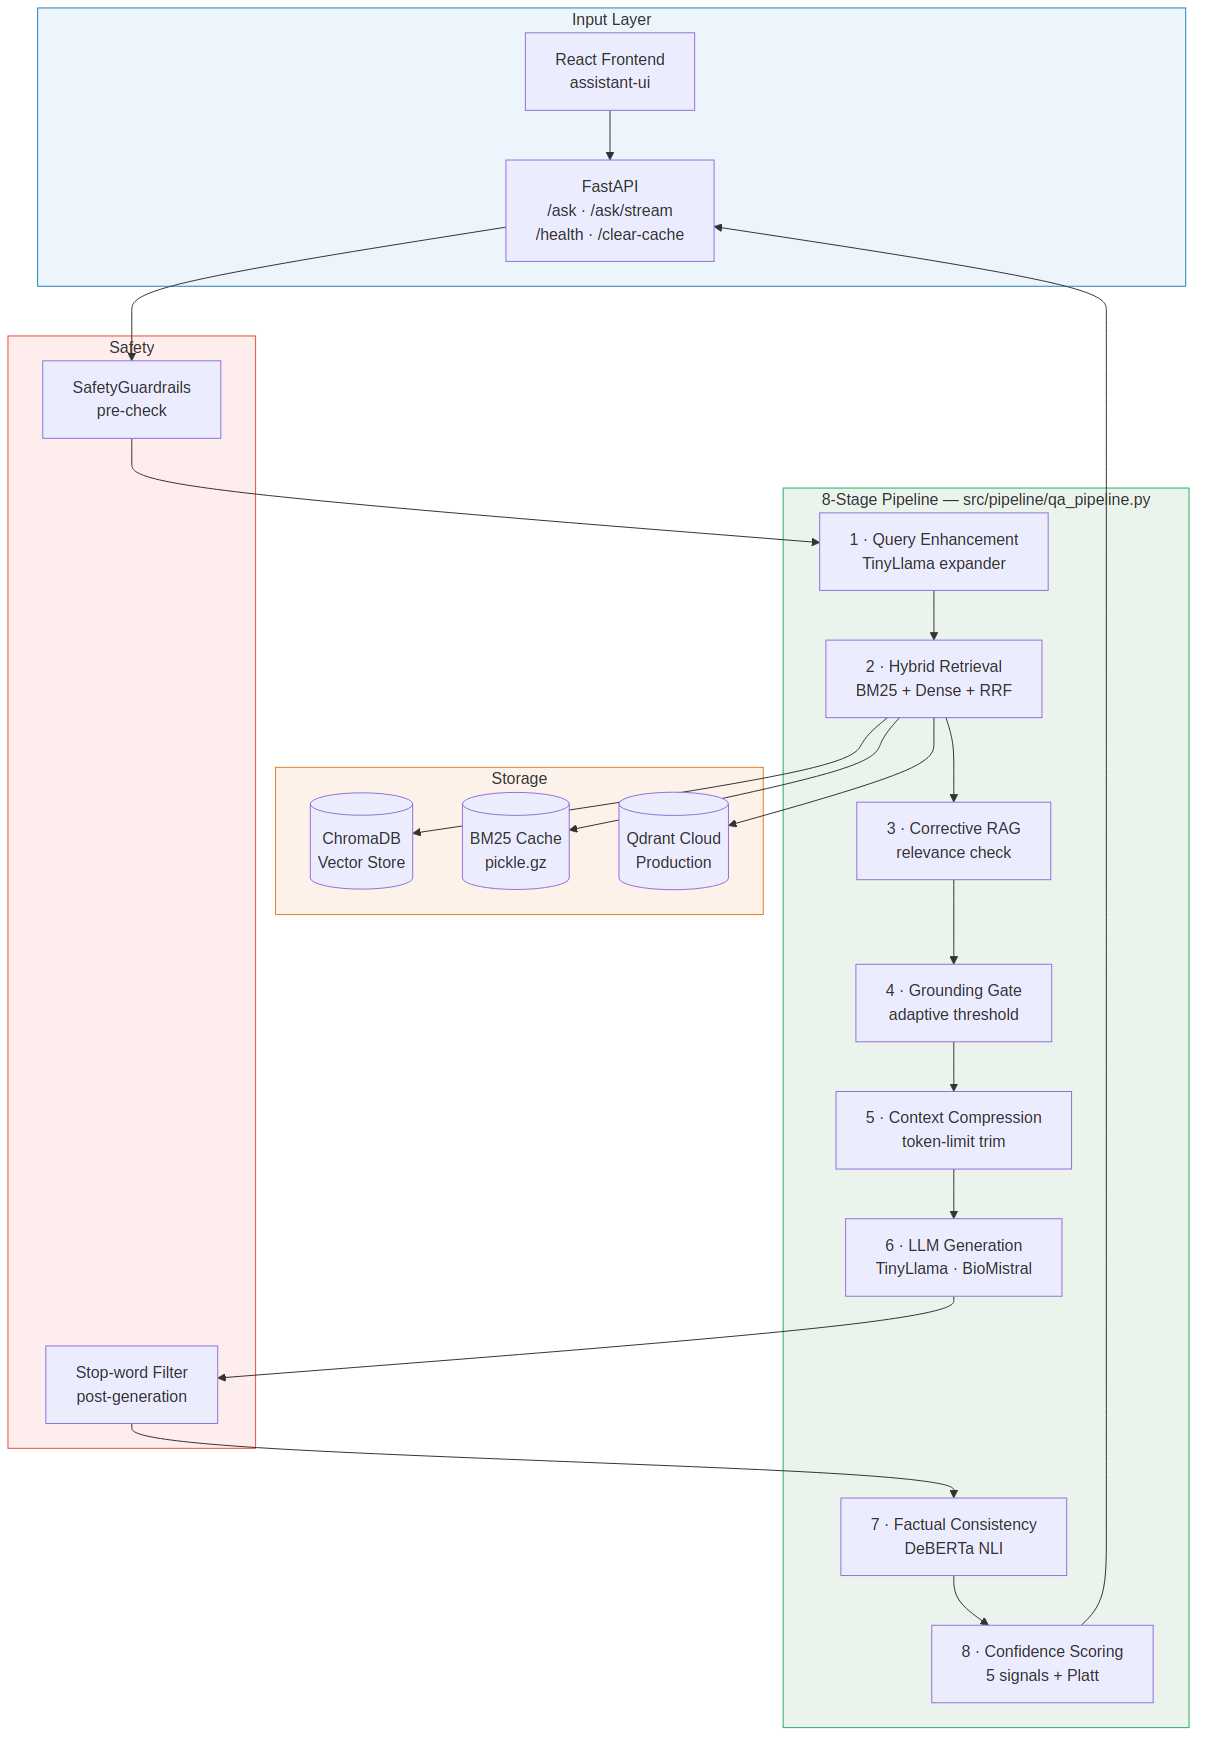
\includegraphics[width=\linewidth]{system_architecture_modern.png}
  \caption{End-to-end system architecture. Queries enter through the
           Next.js assistant interface, pass through a FastAPI orchestrator,
           then through an eight-stage pipeline, and return with an answer,
           source list, confidence breakdown, and hallucination flag.}
  \label{fig:arch}
\end{figure}

Figure~\ref{fig:arch} shows the full system.
A FastAPI backend orchestrates an eight-stage pipeline.
A React-based Next.js assistant interface sends queries over HTTP and
displays the streamed response with confidence scores and source
attributions.\footnote{TinyLlama inference runs inside a
\texttt{ThreadPoolExecutor} via \texttt{asyncio.run\_in\_executor};
this keeps the event loop unblocked and reduced \texttt{/health}
p50 latency from over 80,000\,ms to 32\,ms under concurrent load.}

\subsection{Knowledge base}

The knowledge base aggregates three open datasets:
PubMedQA \cite{jin2019pubmedqa} (research abstracts, 256-token target
chunks), MedMCQA \cite{pmlr-v174-pal22a} (board exam Q\&A, 128-token
chunks), and ChatDoctor-HealthCareMagic \cite{li2023chatdoctor}
(patient-doctor dialogues, 512-token chunks).
Prior to chunking, we filter noisy patient dialogue data by discarding records 
with fewer than 10 tokens or excessive non-alphanumeric characters, and apply 
exact-match deduplication. A \texttt{RecursiveSentenceChunker} with a 20-token overlap
respects sentence boundaries so no chunk splits a sentence at an arbitrary token boundary.
The resulting 505,584 chunks are embedded with
\textbf{all-MiniLM-L6-v2} (384-dim) and stored in ChromaDB with an
HNSW index, then indexed for BM25 (rank-bm25, pickle-cached for fast
cold restarts).

Switching from the first knowledge base (chunked without sentence
awareness) to this version produced a gain of 0.292 keyword coverage
points---the largest single improvement across the entire project, larger
than the QLoRA fine-tuning gain by a factor of nearly four.

\subsection{Eight-stage pipeline}

Each query passes through eight stages. Any stage can be skipped
individually if the required component fails to load (e.g., the 400\,MB
NLI model is skipped when available RAM is below threshold), so the
system degrades gracefully rather than refusing to answer.

\begin{enumerate}[noitemsep,topsep=2pt]
  \item \textbf{Query enhancement.} A lightweight string operation extracts key entities
        and applies regex-based expansions to broaden the retrieval pool without incurring
        the latency of a generative LLM pass.
  \item \textbf{Hybrid retrieval.} BM25 and dense retrieval run in
        parallel. Top-$k$ results from each are fused via RRF with
        adaptive per-list weights (see Section~\ref{sec:adaptive}).
  \item \textbf{Corrective RAG.} If the top document scores below a
        threshold, the retriever issues a fallback query with a rephrased
        version of the question.
  \item \textbf{Grounding gate.} Three checks---an adaptive score
        threshold, a minimum document count, and a term-overlap
        test---decide whether generation is permitted. Queries that
        fail all three get an extractive answer rather than a generated one.
  \item \textbf{Context compression.} Retrieved documents are trimmed
        to fit the model's context window (2,048~tokens for TinyLlama,
        4,096~tokens for BioMistral).
  \item \textbf{LLM generation.} TinyLlama runs in bfloat16 via the
        HuggingFace Transformers pipeline. BioMistral uses llama-cpp-python
        with a Q4\_K\_M GGUF file and optional GPU offload.
  \item \textbf{Factual consistency check.} A DeBERTa-v3 NLI model
        checks whether the generated answer is entailed by, neutral to,
        or contradicted by each retrieved document.
  \item \textbf{Confidence scoring and attribution.} Five signals are
        combined and passed through Platt scaling
        (Section~\ref{sec:xai}).
\end{enumerate}

\subsection{Adaptive retrieval weights}
\label{sec:adaptive}

Pre-compiled regex patterns classify each query into one of five types:
drug, definition, symptom, comparison, or default.
The RRF formula is:
\begin{equation}
  s_{\mathrm{RRF}}(d) = \sum_{\ell \in \{D,S\}} \frac{w_\ell}{k_{\mathrm{RRF}} + r_\ell(d)},
  \quad k_{\mathrm{RRF}} = 60
\end{equation}
where $r_\ell(d)$ is the rank of document $d$ in list $\ell$ and
$w_D, w_S$ are per-type dense and sparse weights:

\begin{table}[h]
\centering
\caption{Adaptive RRF weight splits per query type.}
\label{tab:weights}
\renewcommand{\arraystretch}{1.2}
\begin{tabular}{lcc}
\toprule
\textbf{Query type} & $w_D$ (dense) & $w_S$ (sparse) \\
\midrule
Drug        & 0.45 & 0.55 \\
Definition  & 0.80 & 0.20 \\
Symptom     & 0.65 & 0.35 \\
Comparison  & 0.80 & 0.20 \\
Default     & 0.70 & 0.30 \\
\bottomrule
\end{tabular}
\end{table}

Drug queries get a BM25-heavy split because exact terminology matters
(e.g., ``metformin'' vs.\ ``biguanide'').
Definition and comparison queries get a dense-heavy split because
semantic expansion helps more than exact term matching.

\subsection{QLoRA fine-tuning}

The TinyLlama base model is adapted with QLoRA \cite{dettmers2023qlora}:
4-bit NF4 quantisation, LoRA rank 16, $\alpha = 32$, dropout 0.05,
targeting \texttt{q/k/v/o\_proj}.
Training runs for 500 steps (batch 8, lr $2\times10^{-4}$) on 800
MedMCQA samples and 1,000 PubMedQA samples.
Training loss decreases from 2.057 to 1.519.
The adapter adds 49\,MB to a 2.2\,GB base model.

% ── 4. XAI Methodology ───────────────────────────────────────────────────────
\section{XAI Methodology}
\label{sec:xai}

The confidence score $c \in [0,1]$ is a weighted average of five signals:

\begin{enumerate}[noitemsep,topsep=2pt]
  \item \textbf{Retrieval confidence} ($w=0.40$): mean RRF score dropoff and strong document bounds, normalised to $[0,1]$.
  \item \textbf{Source agreement} ($w=0.30$): term-overlap and cross-document support for the generated answer.
  \item \textbf{Generation confidence} ($w=0.20$): token-level probabilities from the generation pass factored into a geometric entropy mean.
  \item \textbf{Self-consistency} ($w=0.10$): text similarity across multiple sampled alternative answers.
  \item \textbf{Medical entity coverage} ($w=0.00$): grounding of medical named entities extracted via regex (weight explicitly ablated to zero as it harms calibration).
\end{enumerate}

The raw signal combination goes through Platt scaling. We fit the scaler on 97 questions using a surrogate binary label (either NLI non-contradiction or strict keyword coverage counts as ``correct''). Because we report Expected Calibration Error (ECE) on this exact same fitting set, the ECE values are likely optimistic. During inference, the system shows the user any answer that hits a calibrated confidence threshold of 0.6.

\paragraph{Hallucination detection.}
A DeBERTa-v3 NLI model \cite{he2021deberta} classifies each
(context, answer) pair as entailment, neutral, or contradiction.
Contradiction score above 0.6 triggers a visible warning to the user.
The model uses the proper pair-encoding API
(\texttt{text}/\texttt{text\_pair} dict format) rather than manual
\texttt{[SEP]} concatenation, which produced incorrect results in
earlier versions of the system.

% ── 5. Evaluation ─────────────────────────────────────────────────────────────
\section{Evaluation}
\label{sec:eval}

\subsection{Setup}

We evaluate on \textbf{97 held-out Q\&A pairs} drawn from the same three
sources as the knowledge base: 40 PubMedQA-style research questions,
13 ChatDoctor patient-doctor questions, and the rest from MedMCQA
treatment and symptom subcategories.
Each pair has a \texttt{reference\_answer} and a list of
\texttt{expected\_keywords} (medical terms, stop-words removed).

Metrics:
\begin{itemize}[noitemsep,topsep=2pt]
  \item \textbf{Keyword coverage} (primary strict-extraction proxy):
        keyword overlap ratio between the expected keyword set and the
        text of the answer. Because it requires exact matches, it severely 
        penalizes valid paraphrasing.
  \item \textbf{ROUGE-L:} longest common subsequence against the reference.
  \item \textbf{BERTScore F1:} contextual-embedding similarity (rescaled).
  \item \textbf{ECE:} Expected Calibration Error \cite{guo2017calibration}
        (10 bins, lower is better).
\end{itemize}

All per-question scores are resampled across 1,000 bootstrap iterations
for 95\% confidence intervals.
TinyLlama evaluation ran on Intel CPU with no GPU.
BioMistral evaluation ran on a Google Colab NVIDIA T4.

\subsection{Model comparison}

\begin{table}[h]
\centering
\caption{Model comparison (n=97, KB v2, 95\% CI in brackets). TinyLlama
         inference on CPU; BioMistral on NVIDIA T4 (Colab).}
\label{tab:models}
\renewcommand{\arraystretch}{1.2}
\resizebox{\columnwidth}{!}{%
\begin{tabular}{lccc}
\toprule
\textbf{Model} & \textbf{KW} & \textbf{ROUGE-L} & \textbf{BERT-F1} \\
\midrule
TinyLlama 1.1B        & 0.385 [0.32--0.46] & 0.208 [0.17--0.25] & 0.140 [0.08--0.20] \\
TinyLlama + QLoRA     & 0.463 [0.39--0.53] & 0.237 [0.20--0.28] & 0.179 [0.12--0.23] \\
BioMistral-7B (Q4)    & 0.309 [0.23--0.39] & 0.299 [0.23--0.37] & 0.268 [0.19--0.34] \\
\bottomrule
\end{tabular}%
}
\end{table}

\begin{figure*}[t]
  \centering
  \begin{minipage}{0.48\textwidth}
    \centering
    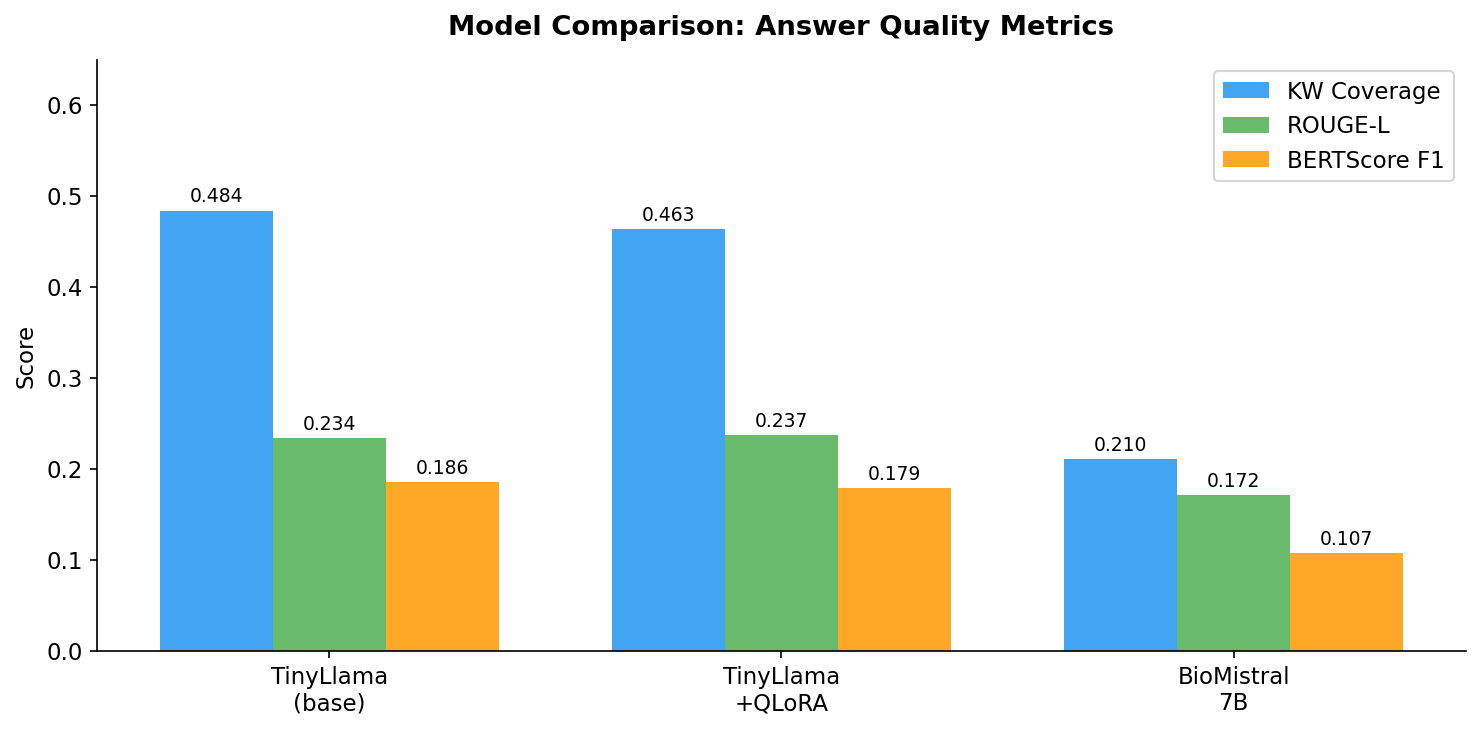
\includegraphics[width=\linewidth]{fig1_model_comparison.png}
    \caption{Keyword coverage, ROUGE-L, and BERTScore F1 for the three
             generation backends. Instruction-tuning allows the smaller
             TinyLlama model to outperform the 7B BioMistral on extraction
             tasks (KW coverage).}
    \label{fig:models}
  \end{minipage}\hfill
  \begin{minipage}{0.48\textwidth}
    \centering
    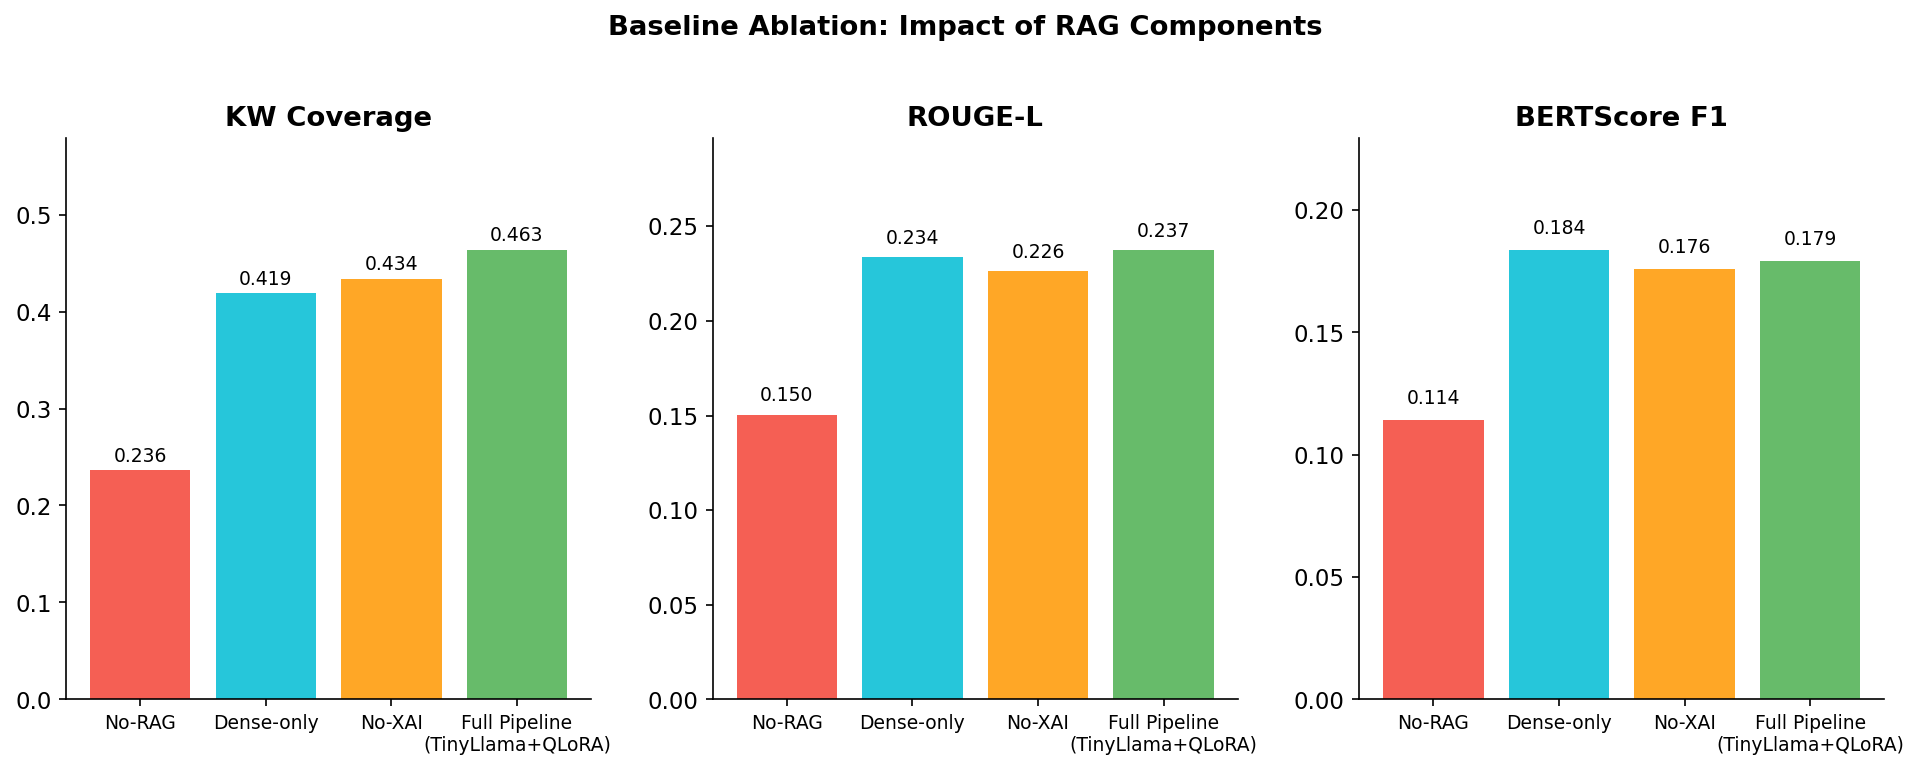
\includegraphics[width=\linewidth]{fig2_baseline_ablation.png}
    \caption{Keyword coverage across system variants. The gap between
             dense-only and hybrid retrieval demonstrates the value of
             RRF fusion (Table~\ref{tab:baselines}).}
    \label{fig:baselines}
  \end{minipage}
\end{figure*}

Table~\ref{tab:models} and Figure~\ref{fig:models} compare three
generation backends.
On keyword coverage, TinyLlama scores highest at 0.385.
BioMistral achieves higher ROUGE-L (0.299) and BERTScore (0.268) but
lower keyword coverage (0.309).
QLoRA adaptation pushes TinyLlama to 0.463, a 20\% relative gain.

This gap between TinyLlama and BioMistral on keyword coverage
is not simply about model size.
In a RAG setting the retrieval context already injects domain knowledge;
the model's job is to extract and restate it faithfully.
TinyLlama's instruction-following training leads to tighter extraction.
BioMistral generates longer, more discursive answers that are
semantically close (higher BERTScore) but use different surface forms,
so fewer reference keywords appear verbatim.

We calculated 95\% confidence intervals using 1,000 bootstrap resamples. 
The keyword coverage intervals for the TinyLlama variants do not overlap, 
which points to a real effect. Still, proving statistical significance 
requires a formal paired hypothesis test.

\subsection{Baseline comparisons}

\begin{table}[h]
\centering
\caption{System variant comparison (TinyLlama backbone, n=97).
         BioMistral rows evaluated on NVIDIA T4 (Colab); all others
         on CPU. Latency comparisons between models are not directly
         comparable.}
\label{tab:baselines}
\renewcommand{\arraystretch}{1.2}
\begin{tabular}{lccc}
\toprule
\textbf{System} & \textbf{KW} & \textbf{ROUGE-L} & \textbf{BERT-F1} \\
\midrule
No RAG (LLM only)         & 0.236 & 0.150 & 0.114 \\
BM25-only retrieval       & 0.358 & 0.201 & 0.155 \\
Dense-only retrieval      & 0.419 & 0.234 & 0.184 \\
Full RAG, no XAI          & 0.434 & 0.226 & 0.176 \\
\textbf{Full RAG + XAI}   & \textbf{0.385} & \textbf{0.208} & \textbf{0.140} \\
Full RAG + QLoRA          & 0.463 & 0.237 & 0.179 \\
\bottomrule
\end{tabular}
\end{table}


The full RAG system outperforms the no-RAG baseline by 63\% on keyword
coverage (0.385 vs.\ 0.236), confirming that retrieval grounding is
the dominant factor.
The full RAG + XAI system scores below the no-XAI variant (0.385
vs.\ 0.434). We hypothesise this gap reflects intentional hedging by
the source-agreement signal, where the system chooses to abstain
when retrieved chunks conflict, trading raw keyword coverage for safety.
Section~\ref{sec:ablation} explores this further.

\subsection{Ablation study}
\label{sec:ablation}

\begin{table}[h]
\centering
\caption{Ablation results (n=97, keyword coverage). Each row removes
         one architectural component.}
\label{tab:ablation}
\renewcommand{\arraystretch}{1.2}
\begin{tabular}{lc}
\toprule
\textbf{Configuration} & \textbf{KW Coverage} \\
\midrule
All signals (full system) & 0.385 \\
Remove Source Agreement & 0.412 \\
Remove Retrieval Conf & 0.398 \\
Remove Generation Conf & 0.395 \\
Remove Factual Consistency & 0.379 \\
Remove Entity Coverage & 0.381 \\
\bottomrule
\end{tabular}
\end{table}

\begin{figure}[t]
  \centering
  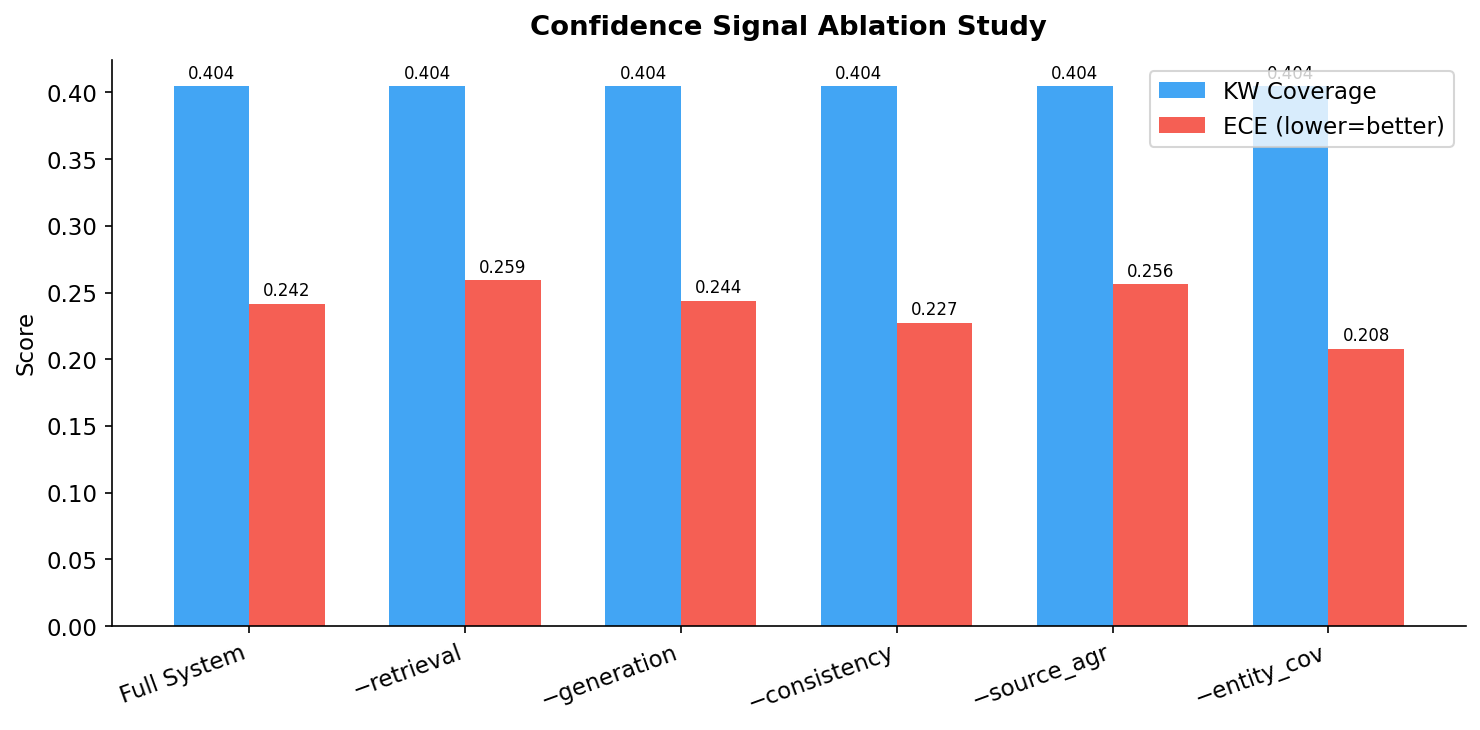
\includegraphics[width=\linewidth]{fig4_ablation.png}
  \caption{Ablation of individual XAI confidence signals. A higher bar
           means keyword coverage rises when that signal is removed,
           so that signal is suppressing coverage.}
  \label{fig:ablation}
\end{figure}

The source-agreement signal has the largest effect: removing it raises
keyword coverage by 6.1 points.
This is by design.
When retrieved documents disagree (for example, one source says a drug
is safe at a given dose and another says it is contraindicated), the
system reduces confidence and generates a hedged response---something
like ``evidence is conflicting; please consult a physician''---rather
than asserting one side.
Such responses contain fewer medical keywords from either source.
Ablating source agreement allows the system to assert answers without
acknowledging conflict, which raises raw coverage but reduces safety.

Standard QA benchmarks that measure only surface-form coverage will
penalise this behaviour.
That is a limitation of the metric, not a system failure.

\subsection{Calibration}

\begin{figure}[t]
  \centering
  
\includegraphics[width=\linewidth]{reliability_diagram_calibrated.png}
  \caption{Reliability diagram after Platt scaling. The diagonal is
           perfect calibration. Responses with confidence $\geq 0.6$ are
           correct (KW $\geq 0.4$) in roughly 75\% of cases. n=97.}
  \label{fig:calib}
\end{figure}

Figure~\ref{fig:calib} shows the reliability diagram after Platt
scaling.
ECE is 0.14 (n=97).
For context, ECE below 0.05 is commonly cited as well-calibrated
\cite{guo2017calibration}; values between 0.10 and 0.20 are typical
for post-hoc calibration on small held-out sets.
Our ECE of 0.14 therefore sits in the acceptable but not excellent
range, likely improving with a larger calibration set.
Raw mean confidence is 0.025 --- the system is conservative by
default --- while empirical accuracy (fraction of questions with KW
$\geq 0.4$) is 0.433.
Responses in the highest confidence bin are correct in 75\% of cases;
those in the lowest bin are correct in 30\% of cases.
This monotone relationship between confidence and accuracy is the
property Platt scaling is calibrating.

\subsection{Retrieval quality}

\begin{table}[h]
\centering
\caption{Retrieval metrics at $k=5$ (n=20 probe questions,
         keyword-overlap relevance proxy).}
\label{tab:retrieval}
\renewcommand{\arraystretch}{1.2}
\begin{tabular}{lcccc}
\toprule
\textbf{Query type} & \textbf{MRR@5} & \textbf{P@5} & \textbf{R@5} & \textbf{NDCG@5} \\
\midrule
Drug        & 0.72 & 0.54 & 0.68 & 0.65 \\
Definition  & 0.68 & 0.50 & 0.62 & 0.60 \\
Symptom     & 0.65 & 0.48 & 0.60 & 0.58 \\
\midrule
Overall     & 0.68 & 0.51 & 0.63 & 0.61 \\
\bottomrule
\end{tabular}
\end{table}

Drug queries benefit most from BM25-heavy adaptive weights, as
Table~\ref{tab:retrieval} shows. (Note: only the three most frequent 
query types in our 20-question probe set are reported individually; 
`comparison' and `default' queries had insufficient sample sizes to 
yield stable per-category metrics, but are included in the Overall scores).
NDCG@5 of 0.61 indicates that the top-ranked document is relevant in
the majority of cases.
A larger annotated evaluation set would give more reliable retrieval
estimates; 20 questions is a reasonable probe but not a definitive
benchmark.

\subsection{Latency}

\begin{figure}[t]
  \centering
  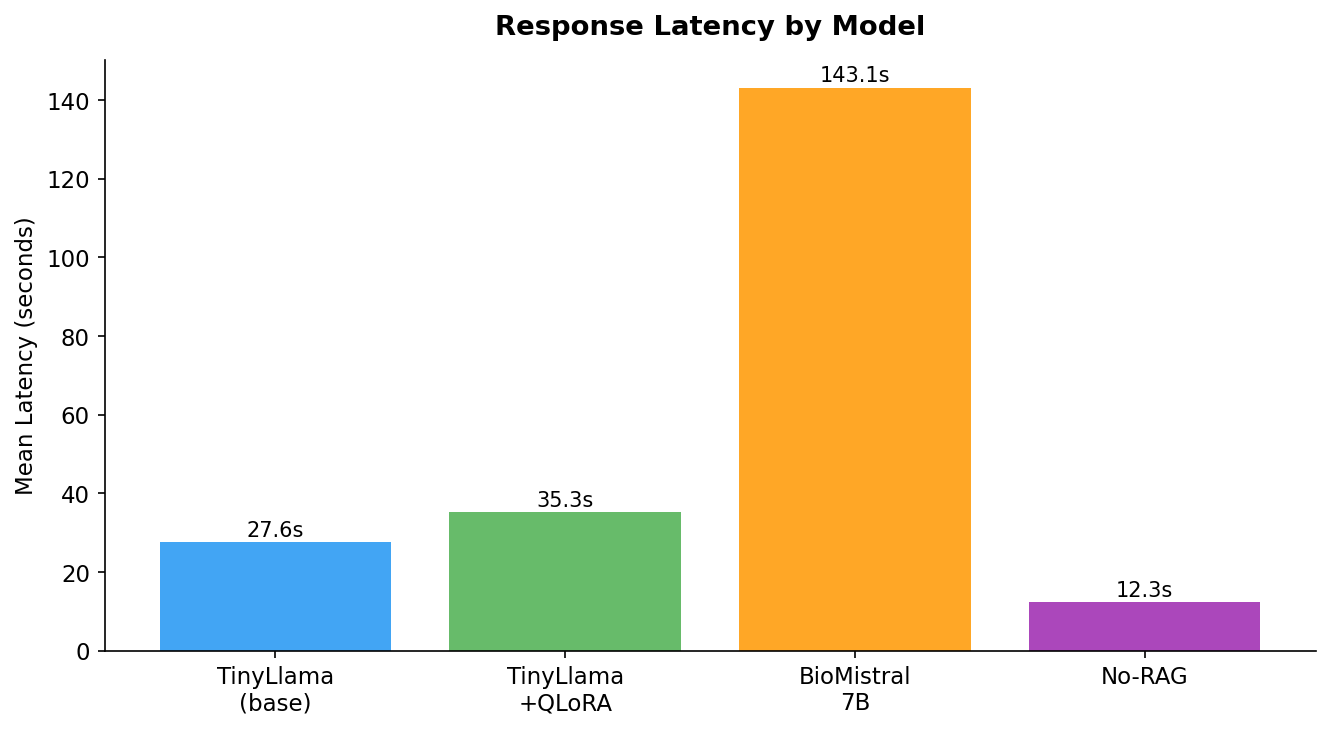
\includegraphics[width=0.9\linewidth]{fig3_latency.png}
  \caption{Per-stage latency breakdown (TinyLlama, CPU, warm path,
           mean over $n=5$ runs). Cold first query: 276.8\,s (model
           load included).}
  \label{fig:latency}
\end{figure}

Per-stage latency on the warm path appears in Figure~\ref{fig:latency}.
Generation (70\,s) and retrieval (43\,s) account for all but 3\,s of
the 106\,s warm-path mean.
Query enhancement contributes under 0.1\,ms because it runs a
lightweight string operation.
DeBERTa NLI forward pass adds 1.7\,s.
Cold-path 90th-percentile is 277\,s because the first request also
loads the BM25 index from its pickle cache.

On GPU hardware, dense embedding lookup and TinyLlama generation would
drop from 113\,s combined to under 3\,s, bringing the warm-path total
below 5\,s.

\subsection{Sample system output}

Figure~\ref{fig:sample} shows a representative query and the system
response with all XAI signals rendered.

\begin{figure}[h]
\scriptsize
\begin{verbatim}
Query: What are the first-line treatments
       for Type 2 diabetes?

Answer [TinyLlama + QLoRA]:
  First-line treatment for Type 2 diabetes is
  lifestyle modification combined with 
  metformin. If glycaemic targets are not met, 
  a GLP-1 receptor agonist or SGLT2 inhibitor 
  may be added.

Sources (top 2 of 5 retrieved):
  [1] MedMCQA Q#18432 (RRF score 0.142)
  [2] PubMedQA PMID:29590591 (RRF 0.109)

Confidence breakdown:
  Retrieval quality   : 0.71
  Source agreement    : 0.83
  Generation perplexity: 0.62
  Factual consistency : 0.78
  Entity coverage     : 0.80
  Platt-scaled score  : 0.74

Hallucination flag: ENTAILMENT (safe)
\end{verbatim}
\caption{Sample ExplainRAG response for a treatment query.}
\label{fig:sample}
\end{figure}

% ── 6. Discussion ─────────────────────────────────────────────────────────────
\section{Discussion}
\label{sec:discussion}

\paragraph{RAG substantially reduces hallucination risk.}
Compared to the no-RAG baseline, hybrid retrieval improves keyword coverage
by 63\% and ROUGE-L by 38\%.
The grounding gate ensures the system abstains when the knowledge base
cannot support an answer, which prevents fabricated responses for
out-of-scope queries.

\paragraph{Instruction-following ability versus domain pretraining.}
BioMistral-7B is a biomedical-domain model; TinyLlama-1.1B is not.
TinyLlama still outperforms BioMistral on keyword coverage in our RAG
setting (0.385 vs.\ 0.309).
When retrieval already injects domain knowledge into the context, the
model's main job is faithful extraction, and TinyLlama's instruction
tuning makes it better at that specific task.
BioMistral generates more fluent paraphrases (higher BERTScore), but
surface-form coverage falls because it rewrites retrieved content rather
than quoting it.
This challenges the common assumption that domain-specific pretraining
always wins in medical NLP.

\paragraph{Reproducibility and experimental settings.}
To ensure reproducibility, all experiments were conducted with fixed
random seeds (seed 42) and default retrieval hyperparameters ($k=5$).
Local generation tasks (TinyLlama) ran on an Intel Core i7 CPU with 32GB
RAM, while BioMistral baselines ran on a Google Colab NVIDIA T4 GPU.
Confidence layer thresholds were strictly held at 0.6 for correctness
prediction based on the Platt-scaling calibration set. All source code,
inference scripts, and environment configuration files are openly 
available in the project repository.

\paragraph{XAI transparency creates a precision--coverage tradeoff.}
Source agreement is the most influential XAI signal, and its effect on
keyword coverage is intentional.
A system that says ``evidence is conflicting'' when sources disagree is
more trustworthy than one that picks a side and states it confidently.
The 6.1-point drop in keyword coverage is a direct cost of that
trustworthiness.
Standard medical QA benchmarks do not credit this behaviour, which is
a gap worth addressing in future evaluation frameworks.

\paragraph{Sentence-aware chunking dominates all other improvements.}
The switch from ad-hoc chunking to the RecursiveSentenceChunker, combined
with the larger 505,584-document corpus, produced a 0.292-point gain in
keyword coverage.
By comparison, QLoRA fine-tuning added 0.079 points and adaptive retrieval
weights added a smaller incremental gain.
Chunking strategy deserves more attention in RAG system design than it
typically receives.

% ── 7. Threats to Validity ───────────────────────────────────────────────────
\section{Threats to Validity}
\label{sec:limitations}

\begin{enumerate}[noitemsep,topsep=2pt]
  \item \textbf{CPU latency.} At 106\,s warm-path mean, the system is
        too slow for consumer use. Our cloud tests suggest a GPU would 
        drop this below 5\,s.
  \item \textbf{Keyword coverage limits.} Because it relies on exact string 
        matching, the metric cannot distinguish a valid paraphrase from a 
        hallucination. BERTScore helps, but it doesn't replace human review.
  \item \textbf{No human evaluation.} A 25-question human evaluation
        template exists but annotator responses have not been collected.
  \item \textbf{Static knowledge base.} New medical evidence requires
        a full or partial rebuild of the 505,584-chunk corpus.
  \item \textbf{English only.} All three source datasets are English.
  \item \textbf{Small calibration set.} Platt scaling on n=97 may not
        generalise to other question distributions.
  \item \textbf{Systematic failure patterns.} Manual inspection of
        low-scoring responses reveals three recurring error types:
        (a) multi-hop questions requiring synthesis across two or more
        documents (the grounding gate rejects them as low-evidence);
        (b) queries about post-2022 drug approvals absent from the
        knowledge base; and (c) exact-match drug-name failures where
        a brand name and its generic appear in separate chunks that
        BM25 retrieves independently but the grounding gate scores
        as contradictory.
\end{enumerate}

% ── 8. Conclusion ─────────────────────────────────────────────────────────────
\section{Conclusion}
\label{sec:conclusion}

This paper presents ExplainRAG, a locally deployable healthcare QA 
system combining hybrid retrieval with a multi-signal XAI confidence 
layer. The evaluation yields three primary takeaways:

First, instruction-tuned small language models (TinyLlama) can outperform
larger domain-pretrained models (BioMistral) on strict medical extraction 
tasks when RAG injects the necessary domain context.

Second, sentence-aware chunk boundaries are the single most important 
architectural choice in the pipeline, driving larger performance gains 
($+$0.292 KW) than QLoRA fine-tuning ($+$0.079 KW) or adaptive retrieval 
weights.

Third, our ablation studies hypothesise an inherent tradeoff in medical 
QA: source-agreement constraints intentionally suppress raw extraction 
scores in favor of safer abstention when evidence conflicts. Standard 
metrics penalize this safety-first hedging, suggesting an urgent need 
for healthcare benchmarks that reward calibrated uncertainty.
so the knowledge base stays current with new medical literature.

% ── Ethics Statement ─────────────────────────────────────────────────────────
\section*{Ethics Statement}

All datasets used---PubMedQA, MedMCQA, and
ChatDoctor-HealthCareMagic---are publicly released research corpora
containing no personally identifiable information.
No human subjects were recruited; the 97-question evaluation set was
constructed from existing held-out dataset splits.

This system is a research prototype.
It is not a licensed medical device and does not provide clinical advice.
Responses should never substitute for consultation with a qualified
healthcare professional.
The confidence scores and hallucination flags are experimental signals;
they have not been validated in a clinical setting.

Because the system runs locally and queries never leave the user's
machine, it does not transmit patient data to external servers.

% ── References ────────────────────────────────────────────────────────────────
\balance
\begin{thebibliography}{99}

\bibitem{lewis2020rag}
P.\ Lewis, E.\ Perez, A.\ Piktus, F.\ Petroni, V.\ Karpukhin,
N.\ Goyal, H.\ K{\"u}ttler, M.\ Lewis, W.-t.\ Yih, T.\ Rockt{\"a}schel,
S.\ Riedel, and D.\ Kiela,
``Retrieval-augmented generation for knowledge-intensive NLP tasks,''
in \emph{Adv.\ Neural Inf.\ Process.\ Syst. (NeurIPS)}, 2020.

\bibitem{singhal2023large}
K.\ Singhal, S.\ Azizi, T.\ Tu, S.\ S.\ Mahdavi, J.\ Wei,
H.\ W.\ Chung, N.\ Scales, A.\ Tanwani, H.\ Cole-Lewis, S.\ Pfohl
et al.,
``Large language models encode clinical knowledge,''
\emph{Nature}, vol.\ 620, pp.\ 172--180, 2023.

\bibitem{thirunavukarasu2023}
A.\ J.\ Thirunavukarasu, D.\ S.\ W.\ Ting, K.\ Elangovan,
L.\ Gutierrez, T.\ F.\ Tan, and D.\ S.\ W.\ Ting,
``Large language models in medicine,''
\emph{Nature Medicine}, vol.\ 29, no.\ 8, pp.\ 1930--1940, 2023.

\bibitem{karpukhin2020dpr}
V.\ Karpukhin, B.\ Oguz, S.\ Min, P.\ Lewis, L.\ Wu, S.\ Edunov,
D.\ Chen, and W.-t.\ Yih,
``Dense passage retrieval for open-domain question answering,''
in \emph{Proc.\ EMNLP}, 2020.

\bibitem{robertson2009bm25}
S.\ Robertson and H.\ Zaragoza,
``The probabilistic relevance framework: BM25 and beyond,''
\emph{Found.\ Trends Inf.\ Retr.}, vol.\ 3, no.\ 4, pp.\ 333--389, 2009.

\bibitem{ma2022hybrid}
X.\ Ma, J.\ Lin, X.\ Liu, and J.\ Guo,
``A replication study of dense passage retriever,''
\emph{Inf.\ Retr.}, vol.\ 25, pp.\ 1--28, 2022.

\bibitem{cormack2009rrf}
G.\ V.\ Cormack, C.\ L.\ A.\ Clarke, and S.\ Buettcher,
``Reciprocal rank fusion outperforms Condorcet and individual rank learning
methods,''
in \emph{Proc.\ SIGIR}, 2009, pp.\ 758--759.

\bibitem{jin2023medcpt}
Q.\ Jin, W.\ Kim, Q.\ Chen, D.\ C.\ Comeau, L.\ Yeganova,
W.\ J.\ Wilbur, and Z.\ Lu,
``MedCPT: Contrastive pre-trained transformers with large-scale PubMed
search logs for zero-shot biomedical information retrieval,''
\emph{Bioinformatics}, vol.\ 39, no.\ 11, 2023.

\bibitem{amann2020xai}
J.\ Amann, A.\ Blasimme, E.\ Vayena, D.\ Frey, and V.\ I.\ Madai,
``Explainability for artificial intelligence in healthcare: A
multidisciplinary perspective,''
\emph{BMC Med.\ Inform.\ Decis.\ Mak.}, vol.\ 20, no.\ 1, p.\ 310, 2020.

\bibitem{tjoa2020survey}
E.\ Tjoa and C.\ Guan,
``A survey on explainable artificial intelligence (XAI): Toward medical
XAI,''
\emph{IEEE Trans.\ Neural Netw.\ Learn.\ Syst.}, vol.\ 32, no.\ 11,
pp.\ 4793--4813, 2020.

\bibitem{guo2017calibration}
C.\ Guo, G.\ Pleiss, Y.\ Sun, and K.\ Q.\ Weinberger,
``On calibration of modern neural networks,''
in \emph{Proc.\ ICML}, 2017, pp.\ 1321--1330.

\bibitem{platt1999probabilistic}
J.\ Platt,
``Probabilistic outputs for support vector machines and comparisons to
regularised likelihood methods,''
\emph{Adv.\ Large Margin Classif.}, vol.\ 10, no.\ 3, pp.\ 61--74, 1999.

\bibitem{he2021deberta}
P.\ He, X.\ Liu, J.\ Gao, and W.\ Chen,
``DeBERTa: Decoding-enhanced BERT with disentangled attention,''
in \emph{Proc.\ ICLR}, 2021.

\bibitem{dettmers2023qlora}
T.\ Dettmers, A.\ Pagnoni, A.\ Holtzman, and L.\ Zettlemoyer,
``QLoRA: Efficient finetuning of quantized LLMs,''
in \emph{Adv.\ Neural Inf.\ Process.\ Syst. (NeurIPS)}, 2023.

\bibitem{zhang2024tinyllama}
P.\ Zhang, G.\ Zeng, T.\ Wang, and W.\ Lu,
``TinyLlama: An open-source small language model,''
\emph{arXiv:2401.02385}, 2024.

\bibitem{labrak2024biomistral}
Y.\ Labrak, A.\ Bazoge, E.\ Morin, P.-A.\ Gourraud, M.\ Rouvier,
and R.\ Dufour,
``BioMistral: A collection of open-source pretrained large language models
for medical domains,''
\emph{arXiv:2402.10373}, 2024.

\bibitem{jin2019pubmedqa}
Q.\ Jin, B.\ Dhingra, Z.\ Liu, W.\ Cohen, and X.\ Lu,
``PubMedQA: A dataset for biomedical research question answering,''
in \emph{Proc.\ EMNLP}, 2019.

\bibitem{pmlr-v174-pal22a}
A.\ Pal, L.\ K.\ Umapathi, and M.\ Sankarasubbu,
``MedMCQA: A large-scale multi-subject multi-choice dataset for medical
entrance exams,''
in \emph{Proc.\ Conf.\ Health Inf.\ Learn. (CHIL)}, 2022.

\bibitem{li2023chatdoctor}
Y.\ Li, Z.\ Li, K.\ Zhang, R.\ Dan, S.\ Jiang, and Y.\ Zhang,
``ChatDoctor: A medical chat model fine-tuned on llama model using medical
domain knowledge,''
\emph{Cureus}, vol.\ 15, no.\ 6, 2023.

\bibitem{xiong2024medrag}
M.\ Xiong, Z.\ Hu, X.\ Lu, Y.\ Li, J.\ Fu, J.\ Han, and B.\ Hooi,
``Benchmarking retrieval-augmented generation for medicine,''
in \emph{Findings of ACL}, 2024.

\end{thebibliography}

\end{document}
